% Sample file for 'CACM - Research Highlights'-type articles
% Created by: Gerry Murray, Elec. Pub. Info. Mgr., Pubs. Dept., ACM HQ, NY.
% (murray@hq.acm.org)
%
% This is "research-highlights-sample.tex" (sample file) V1.1 Sept. 2008
% This file should be compiled with V1.1 of "research4cacm.cls" Sept. 2008
%
% If you have already submitted an article to an ACM/SIGS Conference, and have had your
% article published in one of the 'Proceedings', then you have probably used
% the (ACM/SIGS) 'sig-alternate' class and .tex file.
% Any such 'conference-prepared' source .tex file is 'compatible' with the class file
% 'research4cacm' which you will use to prepare your article for inclusion in the magazine 'CACM'.
%
% Here are the steps to take in order to 'morph' your article from being
% a 'conference' article to one more suitable for inclusion in 'Communications of the ACM'.
%
% 1. Change \documentclass{sig-alternate}  to \documentclass{research4cacm}
%
% 2. Comment out the conference information e.g.  %\conferenceinfo{WOODSTOCK}{'97 El Paso, Texas USA}
%
% 3. Make sure the copyright data is correct e.g. \crdata{0001-0782/08/0200}
%
% 4. Make sure the YEAR is correct e.g. \CopyrightYear{2008} with the current default being �2008�.
%
% 5. Comment out the Classification scheme, general terms and keywords.
%
% 6. If you have mentioned authors in the 'Additional Authors' section you should
%    'move them back' into the byline (so that they appear with all the other authors).
%    ALL authors, in Research Highlights articles, get equal billing.
%
% 7. Suitably edit the file (i.e. body text) so as to make it more appropriate for a wider audience.
%
% If, early on in the editorial process, the 'correct' copyright data becomes available
% please change the copyright data to suit, otherwise leave the default '0001-0782/08/0X00'.
% (The editorial staff will change it later on in the production cycle.)
%
% ================= IF YOU HAVE QUESTIONS =======================
% Technical questions _only_ to
% Gerald Murray (murray@hq.acm.org)
% ===============================================================
% ---------------------------------------------------------------------------------------------------------------
%
\documentclass{research4cacm}
\begin{document}
\newcommand{\E}[2]{\ensuremath{\mathtt{#1_{#2}}}}
\newcommand{\AES}{\E{AES}{256}}
\newcommand{\SHA}{\E{SHA}{256}}
\newcommand{\RSA}{\E{RSA}{1024}}
\newcommand{\MDV}{\E{MD5}{}}
\newcommand{\XOR}{\E{XOR}{}}
\newcommand{\F}[2]{\texttt{#1}(#2)}
\newcommand{\xor}[2]{#1\oplus#2}
\newcommand{\mod}[2]{#1\ \textbf{mod}\ #2}
\newcommand{\sha}[1]{\mod{\F{\SHA}{#1}}{2^{n}}}
\newcommand{\XORkey}{\textsf{\em X\kern -.05em{\raisebox{.2ex}{$\oplus$}\kern -.15em{R\kern +.05em{\raisebox{-.3ex}{\em key}}}}}}
\newcommand{\XORlogo}{\textsf{\em X\kern -.05em{\raisebox{.2ex}{$\oplus$}\kern -.15em{R\kern -1.01em{\raisebox{-1.12ex}{\em key}}}}}}

%
% --- Author Metadata here ---
% Conference information is NOT appropriate for CACM so comment it out.
%\CopyrightYear{2008} % Allows default copyright year (2008) to be over-ridden - IF NEED BE.
%\crdata{0001-0782/08/0X00}  % Allows default copyright data (0001-0782/08/0X00) to be over-ridden - IF NEED BE.
% --- End of Author Metadata ---

\title{Secure Login without Passwords
% \titlenote{(This is a simple titlenote.)For use with research4cacm.cls. Supported by ACM.}
%
% Show use of \thanks - which can appear here (normal/default) or down by the author
\thanks{The original version of this paper is entitled ``XXX" and was
published in (Title of publication, publication date, publisher.)}
}
\subtitle{[An Invention]
%\titlenote{A full version of this paper is available in...}
}
%
% You need the command \numberofauthors to handle the 'placement
% and alignment' of the authors beneath the title.
%
% For aesthetic reasons, we recommend 'three authors at a time'
% i.e. three 'name/affiliation blocks' be placed beneath the title.
%
% NOTE: You are NOT restricted in how many 'rows' of
% "name/affiliations" may appear. We just ask that you restrict
% the number of 'columns' to three.
%
% Use the \alignauthor commands to handle the names
% and affiliations.
%
\numberofauthors{1} %  in this sample file, there are a *total*
% of SIX authors and all of them fit neatly on the first page.
% As said, all authors get 'equal billing' and you should fit all of them on the opening page
% in the 'byline'. The production/editorial-staff will 'separate' names from their affiliations, leaving
% author names beneath the title (in the byline), and moving the affilations/contact information to an area
% after the references at the back of the article.
%
\author{
% You can go ahead and credit any number of authors here,
% e.g. one 'row of three' or two rows (consisting of one row of three
% and a second row of one, two or three).
%
% The command \alignauthor (no curly braces needed) should
% precede each author name, affiliation/snail-mail address and
% e-mail address. Additionally, tag each line of
% affiliation/address with \affaddr, and tag the
% e-mail address with \email.
%
% 1st. author
\alignauthor
Timo Ruiter\titlenote{A note from Dr.~Trovato.}\\
       \affaddr{Terschelling~19}\\
       \affaddr{Heemskerk, The Netherlands}\\
       \email{timo.ruiter@xs4all.nl}
% 2nd. author
%\alignauthor
%G.K.M. Tobin\titlenote{A note from G. Tobin.}\\
%       \affaddr{Institute for Clarity in Documentation}\\
%       \affaddr{P.O. Box 1212}\\
%       \affaddr{Dublin, Ohio 43017-6221}\\
%       \email{webmaster@marysville-ohio.com}
%% 3rd. author
%\alignauthor Lars Th{\o}rv{\"a}ld\titlenote{A note from Lars.}\\
%       \affaddr{The Th{\o}rv{\"a}ld Group}\\
%       \affaddr{1 Th{\o}rv{\"a}ld Circle}\\
%       \affaddr{Hekla, Iceland}\\
%       \email{larst@affiliation.org}
%\and  % use '\and' if you need 'another row' of author names
%% 4th. author
%\alignauthor Lawrence P. Leipuner\\
%       \affaddr{Brookhaven Laboratories}\\
%       \affaddr{Brookhaven National Lab}\\
%       \affaddr{P.O. Box 5000}\\
%       \email{lleipuner@researchlabs.org}
%% 5th. author
%\alignauthor Sean Fogarty\\
%       \affaddr{NASA Ames Research Center}\\
%       \affaddr{Moffett Field}\\
%       \affaddr{California 94035}\\
%       \email{fogartys@amesres.org}
%% 6th. author
%\alignauthor Charles Palmer\\
%       \affaddr{Palmer Research Laboratories}\\
%       \affaddr{8600 Datapoint Drive}\\
%       \affaddr{San Antonio, Texas 78229}\\
%       \email{cpalmer@prl.com}
}

\maketitle
\begin{abstract}
These are the ingredients for secure logins:
\begin{itemize}
\item The website maintains a small array with Secret keys in an HSM, which will be renewed regularly
(oldest key removed, all keys shifted one position, new key added).
\item All cryptographic operations at the website take place in the HSM;
no values are remembered, except Secret keys.
\item For each user, a 128 bit random number acts as the site key for that user.
The user gets a different 128 bit value, which is the \AES\ encryption of the site key for that user with the newest Secret key.
\item Logging in is a process of proving that both the website and the user have the right key by sending hashes of
random 128 bit numbers encrypted with these keys.
Neither the site key nor the user key are ever sent over the line.
\item When Secret keys are changed,
the user automatically gets a new key.
This way, user keys are changed regularly as well.
\item All user keys are put on a keyring,
which is a set of at least 99 keys, each 128 bit long, most of them dummies.
No other information whatsoever is stored in a keyring, which may be stored in an ordinary file.
The keyring may be encrypted with its own keys.
\item The user selects which key is used for what, which it needs to write down or remember.
Although keys themselves are changed regularly,
the key number and its purpose will never change during the lifetime of the keyring, which might be forever.
This makes remembering key numbers, at least for those keys that are used regularly, doable for most people.
\item The keyring itself is something you must have; the key number something you must know,
so logging in using a keyring is a basic form of two-factor authentication.
\end{itemize}
\end{abstract}

\section{Introduction}
Passwords should be kept in memory%
---human memory, that is---%
at all times.
This article is about passwords for websites; the passwords many people use on a day to day basis.
Passwords are an archaic type of security measure
(\cite{Honan2012}),
compared to the scheme proposed here.

\subsection{On human behavior}
The rationale amongst security experts is that passwords should not be written down.
Ever.
And passwords should be unique for each and every website.
Oh, and---I almost forgot---you have to change them as well.
Each month or so will do nicely. 
\par
Yeah, right!
I cannot remember all different passwords I am forced to use, although my memory is quite good.
I \emph{have} to write them down,
	otherwise,
		I am lost.
(Fortunately,
	I have some support for this \cite{Schneier:2005}.)
Therefore,
	I resort to a little black booklet,
		with all my account information.
I don't remember passwords any more,
	I remember where my booklet is.
And I confess that I am compelled to reuse passwords,
	and to keep the ones I am not forced to change,
		so I can actually remember some of them.
So I believe nothing has fundamentally changed in more than 14 years\ldots\cite{Adams:1999:UE:322796.322806}
\par
%Letting humans use passwords is a bad idea because of what humans do:
%forget, steal, conceil, ignore.
%Since their first use they were troublesome,
%which is nicely depicted in the movie WarGames,
%released way back in 1983.
%The `pencil' password for the school's online system was nicely written down on a piece of paper.
%Notice, by the way, that the password was changed regularly!
%\par
I have given up on inventing a scheme for passwords that differ from each other,
can be changed individually at different times, 
and are easy to remember, as not to be forced to write them down.
I believe no such scheme exists, because websites have different requirements regarding passwords.
To see what I mean, watch \cite{youtube:tobyturner}.
\par
For the user, the bad thing with passwords is that you have to keep track of it all.
Remembering difficult passwords is cumbersome for most, and impossible for some.
Tracking things infalliably, and remembering different passwords for each and every site is not something people excel at.

\subsection{A new login approach}
Using a key,
with up to 128 random bits,
to gain access to a website is far more secure than letting people decide which password they would like to use to do so.
\par
This proposed new way of logging in has several advantages over the current practice of websites requiring passwords.
Instead of having to remember dozens of passwords for numerous sites,
you only need to remember a key number for that site, in the range of 1 to 99.
This key number stays the same for that website at all times, so you \emph{can} remember it.

\Section{General description}
This section serves as a general description of the login process,
without going into technical details too much.

\Subsection{A new login scheme}
Userids tend to be in short supply for people with first names like John, Peter, and Chris,
or surnames like Jones or Smith.
This is true for people in almost any country.
And the larger the site, the rarer available userids.
\par
Passwords tend to be weak,
as people choose short, real-life words, like things or names.
Not that people are not willing, but remembering passwords that are too long or too difficult is not easy.
It is very frustrating when you cannot login because you have forgotten your password,
or,
just when you are starting to remember it,
you need to change it again.
\par
As a radical measure, we do away with all this!
\par
Instead of userids, the website holds hashes based on key ring identifiers.
Instead of a password for an account, the website holds one part of a key, of which you have the other part,
like the broken locket Annie clings to in the musical that bears her name.
Your key is different from the key the website has, but they are related to each other.
It is not possible to login with the key that is stored on the website;
you can only login with your personal key, which is verified with the key from the website.
\par
We will let the computers
(yours, the one running the website, and another one dedicated for logins)
do what they do best: compute.
Give them some random bits to chew on, and they are in heaven.
We will let humans (you, your neighbor and your fellow earthlings) do what they do best:
remembering small ordinal numbers.

\Subsection{Storing your keys}
Keys are just long strings of random bits with no information whatsoever.
Your keys are personal and are stored locally.
\par
Imagine a key ring,
	not unlike your own key ring on which you have keys for your car,
		your house,
			shed,
				or locker.
This key ring has a label and 999 keys on it,
	numbered 1 through 999.
Instead of brass or steel,
	these keys are made of 128 random bits each.
The label is another 128 bits long,
	and as random as possible,
		like the keys.
Instead of being on a steel ring,
	these keys,
		with the key ring label,
			are written to a file on disk;
				a blob of 1000 strings of 128 bits.
\par
The use of keys on this key ring is not all that different from using real physical keys.
The bits in a key are comparable with the teeth or holes of a physical key you use to unlock your home.
You do not need to remember exactly how far the teeth need to protrude or exactly where and how deep the holes in your key need to be,
	to be able to unlock the door;
		you just select the right key
			(the whole physical thing at once, with all the right teeth or holes)
				by recognizing its form or its label.

\input{tex/computers-and-links.subsec}

\SubsectionWithoutText{Logging in}
\subsubsection{Part I}
Before starting the login process you select a key from your key ring;
the one you know to belong to the website you are trying to login to.
\par
To login you don't send your key to the server.
Instead, you generate a secret random value,
which you encrypt with your key using a simple \XOR\ operation.
Your key is totally random and the secret random value you encrypt with it is also, well\ldots totally random.
Mixing these random bits gives another totally random value.
The website will receive this value and will try to decrypt this with the key that belongs to your account
%(we will keep you in the dark for now, about how this works).
(as explained in detail below).
When it has decrypted the random login value,
it will know which secret random value you generated.
Instead of telling you the secret random number,
the website sends a hash value of it,
because otherwise someone able to see the network traffic will instantly know your key.
\par
If the website returns a hash value matching your secret random number, you know two things.
First, you know that the website you are talking to can successfully decrypt your random value.
It can only do this if it has a matching key.
Second, you know you are talking to the same site that sent you your key when you applied for an account.
This implies that if you trusted that site then, you can trust this site now, as it can only be the same site.

\subsubsection{Part II}
%This is all great and very sophisticated, but the website wouldn't dare share your wonder about this,
%as you may well fake your enthusiasm, and flatly lie about the correctness of the hash it has sent you.
%To see if your claims hold,
To confirm that you are who you claim to be,
the website will do the same as you and send you an encrypted secret random value.
This cryptogram can only be decrypted by someone owning the right key for the account.
Using \XOR\ with the key you have originally selected from your key ring,
you decrypt it.
Then,
using \XOR\ again,
you combine the two random values you now have,
and return this value to the website.
\par
When the website receives a value matching its secret random number, it knows two things.
First, the user on the other side can successfully decrypt the secret random number.
It can only do this if it has a matching key.
Second, the website knows that this key is from the same key ring that was used when applying for an account.
This implies that if it trusted this user then, it can trust this user now, as it can only be the same user.

\SubsectionWithoutText{Keys}
\subsubsection{On site keys and user keys}
Beware, the icky parts start here (a bit).
\par
When applying for an account, a site key is created by a random generator.
The user key is then computed as the encryption of the site key with a Secret Key, with a block cypher like \AES.
\par
When the user encrypts its secret random value with its key,
it uses \XOR.
This is a very simple and reversible encryption method.
But as both key and value are utterly random, no information is stored in the encrypted value.
The website needs to decrypt the value, and this can only be done with the user key.
But the website does not store user keys,
it stores only site keys\ldots
\par
%The solution to this may be a bit of a dissappointment and a cheat:
The user key is temporarily regenerated by encrypting it again with the Secret Key.
Once the user key is available, the random value can easily be decrypted by \XOR-ing it.
Also, the cryptogram that is sent to the user is a random value \XOR-red with this regenerated user key.
\par
%The clever part,
More important,
however,
is that all the cryptographic functions the website is required to perform take place inside a Hardware Security Module,
or HSM for short.
%Secret Keys can be put in the HSM and made to good use there,
Secret Keys are stored and used in the HSM,
but can never be retrieved from it.
The HSM computes all values needed for the login process,
without ever revealing the keys that are used,
not even to a hacker with full control of the HSM.
\par
In the end,
only random bits enter the HSM,
and only random bits leave it.

\subsubsection{Key lifetime}
%Every key has its lifetime, so Secret Keys need changing every so often, as a good security measure.
As a good security measure, Secret Keys need changing every so often.
The same goes for keys on the user's key ring.
\par
The login protocol is capable of changing keys on the website and keys on the key ring,
without any effort on the user's side.
%Well\ldots, a little program will do it for you, without you noticing.
\par
Logins can be granted,
but new keys may not be,
which results in the expiration of an account.
A website may deny a user new keys when payment is due,
giving users limited login rights.
At any time new keys can be provided again.
\par\vspace{10mm}\noindent
How this all works,
how keys are used,
what a website can do with logins,
and more,
can all be read in the next chapters.

%
% $Header: /usr/local/src/slwp/article/tex/keys.tex,v 1.6 2013/08/28 18:57:52 timo Exp $
%
% AUTHOR:	ing. T.M.C Ruiter
%
\section{Keys}
%The exchanged values in the login process and the keys in a keyring are 128 bits long in this article,
%but could be taken much smaller;
%say,
%16 bits each,
%without doing great injustice to the level of security.
%The use of 128 bits is only a convenient size,
%as it is the \AES\ blocksize, and \SHA\ works with this length naturally.
%This way,
%we take full advantage of their cryptographic power.

\subsection{Secret keys}
\label{sec:secret_keys}
The keys used to encrypt other keys%
---called Secret keys in this article---%
are used to perform \AES\ encryptions of site keys,
and are 256 bits long.
\par
Several Secret keys are used and
are considered to be stored in array $S$, in this article.
With this array, three values are defined.
\begin{enumerate}
\item	The number of stored Secret keys is represented by $m$.
\item	The constant%
\footnote{Although declared a constant, the value of \texttt{MAX\_KEYS} may change over time.
When the login policy regarding the use of old keys is changed, more or fewer old keys will be stored.
For this, \texttt{MAX\_KEYS} needs to be changed.}
\texttt{MAX\_KEYS}, which is the maximum number of keys that will be kept.
The value of $m$ starts at 0 and will reach \texttt{MAX\_KEYS} eventually and grow no more.
The value \texttt{MAX\_KEYS} has a minimum of 2 (a new key and at least 1 old key).
All values in the array $S$ are shifted up one position when a new key is stored, which will always be inserted at $S[0]$.
This way, with at least one key loaded ($m>0$), it always holds that $S[0]$ is the newest key,
and $S[m-1]$ is the oldest key.
With $m>1$, $S[1]$ is the jongest old key.
\item	The constant \texttt{MAX\_ACTIVE\_KEYS},
which is the maximum number of keys that will be used for logging users in.
This value lies in the range $[2, \mathtt{MAX\_KEYS}]$.
\par
Subtracting \texttt{MAX\_ACTIVE\_KEYS} from \texttt{MAX\_KEYS}
gives the number of inactive keys which can be used to reactivate expired user keys.
Users using a user key that is older than the oldest active Secret key cannot login,
but their key can be restored with an inactive Secret key.
If a key is used that is older than the oldest inactive key,
the key cannot be restored and is lost forever.
\end{enumerate}

\subsection{Site keys}
For each user, there exists a site key and a derived user key (see section~\ref{sec:userkeys}).
The site keys are stored in a table of a database,
where the \SHA\ hash of the userid will act as the primary key for that table.
Since the user only sends the \SHA\ hash of its userid, no actual userids will be stored.
\par
Site keys are generated once by a pseudo-random generator, and need never be replaced.
\par
Each time a user tries to login,
the database is queried with the \SHA\ hash of the userid,
and the site key for that user is returned for further processing.

\subsection{User keys}
\label{sec:userkeys}
A user key is computed by encrypting the site key for the user with the joungest (or current) Secret key,
using the \AES\ algorithm.
\par
The keys users get from the website are stored on a keyring (see section \ref{sec:keyring}).
These keys are automatically changed for new keys by the website when the Secret key is changed.

\subsection{Key lifetime and old keys}
For enhanced security, Secret keys need to be replaced at regular intervals.
This change of keys is initiated by the website,
without the possibility to make individual arrangements with any of its users.
\par
After changing the Secret key, it is no longer possible to login with any user key.
Therefore, an array of Secret keys needs to be kept, allowing users to login using an old(er) Secret key.
At least one old Secret key needs to be stored; otherwise, the Secret key cannot be changed without rendering all user keys permanently useless.
\par
Upon successful login with an old key, the user will be provided with a new user key,
with which it can login using the newest Secret key, from that moment on.
Changing of user keys is seamless and the user might, just as well, be kept unaware of this.
\par
The website's security policy should prescribe with what frequency Secret keys are to be changed, and how many old keys should be kept.
If, for instance, the Secret key is changed every month, and 11 old keys are kept, users can still login using a key that is a year old.
If the user key is older than that, the site is not able to verify the user's key any longer.

\subsection{Storing user keys in a keyring}
\label{sec:keyring}
Keys for the user are collected and stored in a keyring.
The keyring is a block of
(at least)
100 random numbers with 128 bits, most of them dummy keys.
The keyring will be considered an array $Z$ in the rest of the article.
Since all bits are entirely random in a keyring%
---for dummies and real keys---%
a keyring stores no information whatsoever.
\par
Real keys in the keyring should be randomly put between the dummy keys.

\subsubsection{Creating a keyring}
A keyring is created by using a random generator of sufficient quality,
which generates 100 random numbers of 128 bits.
Key number zero is used to identify the keyring and will never change after its creation.
The other 99 keys are dummies
(random bits with no meaning whatsoever).
These random numbers are then encrypted and written to a file%
\footnote{A password protected PKCS\#12 file would do nicely.}
on a storage device.
Unencrypted values should never be written to a storage device and only be kept in volatile memory.
It is up to the user to remember how to decrypt its keyring.

\subsubsection{Copying keys and keyrings}
A keyring can be freely copied to other devices, so all keys are available there as well.
The keys of one keyring can be copied to other keyrings, in different locations.
It is up to the user to keep a registration of this.
\par
Encrypted keyrings can be stored in a public place, for easy access, and act as a backup.
A dedicated webserver can be employed for storing encrypted keyrings,
which can be used to restore lost keyrings.
They can also be used to login when away from home with no access to your own keyring.
These temporary keyrings should be discarded when logging out.

\subsubsection{Irretrievably lost keys and keyrings}
When a key number is forgotten and no record of it can be found,
the key must be considered lost.
\par
As the user has supplied websites with personal information,
it may be easy to regain login capabilities by just asking for a new key,
provided a username and maybe some other information can be given.
Selecting a free keynumber on the keyring and replacing that key with the new one should restore the ability to login.
\par
Keyrings can become unusable or lost in two situations:
the device holding it is defective (like a harddisk crash) and no backup has been made,
or the encryption cannot be reversed (PIN forgotten).
In both cases, the user has to start over and create a new keyring, containing only dummy keys.
\clearpage

%
% $Header: /usr/local/src/slwp/article/tex/login.tex,v 1.6 2013/06/19 18:46:16 timo Exp $
%
% AUTHOR:	ing. T.M.C. Ruiter
%
\section{Logging in}
\label{logging_in}
Having unencrypted its keyring, selected a key number ($k$), and entered the userid, the login process can commence.

\subsection{User IDs}
\label{sec:user_ids}
Instead of sending a traditional alphanumeric userid,
we send a hash.
This hash will be used by the webserver to identify the user,
and the webserver will only store hashes in its user database.
This hash is specially crafted,
so guessing will be hard.
\par
The user will still need a userid,
but this userid may be the same%
\footnote{Different userid's for different websites are still possible, but not necessary.
The chosen userid acts like a default userid, or as a password for the keyring, if you like.
The browser may remember the (default) userid for the user.}
for each and every webserver.
The userid is chosen once and can remain the same as long as the keyring exists.
The hash will be constructed using a combination of the userid and the keyring identifyer $Z[0]$.
The hash value that is sent is constructed as follows.
Compute the hash of the keyring identifier:
\[E=mc^2\]
Then replace the most significant bits of $H_0$ with the bit representation of the userid
(a simple string like 'John Doe')
to get $H_0'$.
Then, compute the final 256-bit hash:
\[E=mc^2\]
\par
This hash value is a combination of something the user has
(the keyring)
and something the user knows
(its chosen userid).
This makes it hard to match a stolen set of hashes from a webserver with a set of keyrings from a keyring server.

%%%%%%%%%%%%%%%%%%%%%%%%%%%%%%%%%%%%%%%%%%%%%%%%%%%%%%%%%%%%%%%%%%%
\subsection{Applying for an account}
\label{sec:applying}
When a new user applies for an account,
it presents the webserver with its hash value $U_h$.
Furthermore,
the user should select the index ($d$) of a hitherto unused key
(therefore, a dummy).
\[E=mc^2\]
The user will send $U_h$, along with its dummy key $K_d$ to the webserver.
\par
The webserver will request values for a new user from the login server,
by forwarding the dummy ($K_d$) and
specifying for which website ($W$) the user will be granted access.
The login server will do the following:
\begin{enumerate}
\item First,
	lookup a 256-bit pre-shared key $K_w$,
	which belongs to the website $W$.
\item Generate a 128-bit pseudo-random site key $K_s$ for the user:
\[E=mc^2\]
\item Encrypt the $K_s$ with the current Secret key $S[0]$ to yield the new user key $K_u$,
which is then encrypted with the users dummy key $K_d$:
\[E=mc^2\]
\[E=mc^2\]
\item Finally, the two new values are encrypted with the pre-shared key $K_w$:
\[E=mc^2\]
\[E=mc^2\]
And both are returned to the webserver.
\end{enumerate}
The webserver will then relay the new keys $E_s$ and $E_u$, and $U_h$ to the accounts server.
The accounts server will decrypt those values with it's own pre-shared key $K_w$:
\[E=mc^2\]
\[E=mc^2\]
It will then store the combination of $K_s$ and $U_h$ with the other data it already has for the user,
and the encrypted user key $K_x$ is sent to the user through a separate channel,
like email.
\par
The user can import the new key $K_u$ into the keyring by calculating
\[E=mc^2\]
Finally, with
\[E=mc^2\]
the dummy key $K_d$ at $Z[d]$ is overwritten with the new key $K_u$.

\subsection{Basic login scheme}
The procedure described below to login is the basic login scheme.

%%%%%%%%%%%%%%%%%%%%%%%%%%%%%%%%%%%%%%%%%%%%%%%%%%%%%%%%%%%%%%%%%%%
\subsubsection{Step 1: Knock, knock\ldots}
\label{sec:login_step1}
The user's login program has to compute the folowing:
\begin{enumerate}
\item A pseudo-random number $R_u$ which hash will be returned by the webserver:
\[E=mc^2\]
\item The user key $K_u$ is taken from the keyring at index $k$ and the pseudo-random number is encrypted with it to get the value $A_u$:
\[E=mc^2\]
\[E=mc^2\]
\item The webserver will return a hash value of the user's pseudo-random value.
To be able to verify this hash,
we compute our own hash $B_u$ to verify it with:
\[E=mc^2\]
\end{enumerate}
The special userid hash $U_h$ and the encrypted pseudo-random number $A_u$ are sent to the webserver.

%%%%%%%%%%%%%%%%%%%%%%%%%%%%%%%%%%%%%%%%%%%%%%%%%%%%%%%%%%%%%%%%%%%
\subsubsection{Step 2: Site key lookup and key matching attempts}
\label{sec:login_step2}
The webserver runs a login procedure,
see Algorithm~\vref{alg:webserver_login}.
\par
After receiving $U_h$ from the user, the site key $K_s$ needs to be looked up.
A query with $U_h$ is sent by the webserver to the accounts server.
If a match is found, $K_s$ is returned;
otherwise, $K_s$ is set to zero, indicating that no such record exists.
In the latter case, the values $B_s$ and $P_s$ are both set to zero as well, and returned to the user.
The user needs to rethink its actions and start over.
\par
Now an iterative process starts, trying to find the right Secret key to log the user in.
%The loop runs at most $min(m,\mathtt{MAX\_ACTIVE\_KEYS})$ times.
The webserver will send three values to the login server:
$A_u$,
$K_s$,
and a Secret key index $i$,
starting at 0.
This will be repeated
(increasing index $i$),
until a match is found,
or no more keys can be tried.

%%%%%%%%%%%%%%%%%%%%%%%%%%%%%%%%%%%%%%%%%%%%%%%%%%%%%%%%%%%%%%%%%%%
\subsubsection{Step 3: Login server actions}
\label{sec:login_step3}
The login server is a processor of login values and calls a function of the HSM to compute them
(see Algorithm~\vref{alg:hsm}).
\par
In case $i$ is less than $m$
(the number of stored Secret keys, see section~\vref{sec:secret_keys})
the login server calculates the following, all within the HSM:
\begin{enumerate}
\item Temporarily, regenerate a user key, using the same algorithm as when the key was originally generated:
\[E=mc^2\]
with $S[i]$ the $i$-th Secret key stored in the HSM.
\item With the user key $K_u$, decrypt the pseudo-random the user has sent:
\[E=mc^2\]
\item Calculate a hash with which the user can verify we own the site key $K_s$ and a corresponding Secret key $S[i]$:
\[E=mc^2\]
\item Allowing the user to verify it recieved a trustworthy response,
the webserver may present the user with a certificate stating that it is using a bona fide login server.
This certificate---signed by a common Root CA---contains a public encryption/decryption key.
The private key for the login server ($K_{ls}$) will be stored in its HSM. 
Encrypt $B_s$ with $K_{ls}$:
\[E=mc^2\]
\item To be able to verify that the user owns and knows its user key $K_u$,
is not sending a replay of some earlier succesfull login sequence,
and will be unable to ly about the correctness of the hash of the pseudo-random the webserver will send,
we calculate a challenge for the user.
\par
If the index $i$ equals zero, generate a pseudo-random value
\[E=mc^2\]
otherwise, compute
\[E=mc^2\]
which will be the new key for the user.
\par
We then encrypt $R_s$ to a value $P_s$ the user can decrypt using its key:
\[E=mc^2\]
This value will be different for each time the loop is executed,
even if the same new key is transmitted,
since $K_u$ will change each time.
\item Calculate the expected response also:
\[E=mc^2\]
\end{enumerate}
The HSM will produce the values $B_s$,
$P_s$,
and $Q_s$ as a result of the calculations and the login server will send them back to the webserver,
as an answer to the three values it was given ($A_u$, $K_s$, and $i$).
The HSM will delete all temporary values from memory directly afterwards, and remember only its Secret keys.
\par
Should index $i$ equal $m$, then the array of Secret keys is exhausted.
If we reach this situation, we cannot log the user in since all possible attempts have failed.
Return zero values for $B_s$, $P_s$, and $Q_s$ to indicate this.

%------------------------------------------------------------------
\subsubsection{Step 4: user verifies site key}
\label{sec:login_step4}
The webserver sends $B_s$ and $P_s$ to the user.
If both are zero, the login has failed and the user should return to step 1.
It is advisable for the user to choose different values for the next try.
\par
If $B_s$ contains a nonzero value, the user verifies whether $B_s$ equals $B_u$.
\par
If the two values do not match, the user either has selected the wrong key or uses an old key.
A key can be old if it comes from a keyring that was not used recently.
Another possible reason for a key to be old is when the Secret key of the site has changed recently.
\par
To indicate that no match has been found, we send
\[E=mc^2\]
(128 zeroes) to the webserver.
The webserver will need to start over, and send values $A_u$, $K_s$, and $i+1$ to the login server.
So, back to step 3.

%------------------------------------------------------------------
\subsubsection{Step 5: site verifies user key}
\label{sec:login_step5}
If $B_s$ matches $B_u$, then the webserver has found a Secret key for the user.
The user can now prove it has control over its user key by computing
\[E=mc^2\]
and
\[E=mc^2\]
which is sent to the webserver as proof.
If the webserver accepts $Q_u$ as correct it will log the user in.
\par
If the webserver receives a value $Q_u$ that does \emph{not} match,
something fishy is going on.
Further attempts for this userid, or from that IP address should be scrutinized.

%------------------------------------------------------------------
\subsubsection{Step 6: key replacement}
\label{sec:login_step6}
If this attempt to login was not the first with this key,
the webserver has sent the user a new key in $R_s$ (instead of a pseudo-random value).
The user should store this new key in the keyring, overwriting the old key the user has just used.

%%%%%%%%%%%%%%%%%%%%%%%%%%%%%%%%%%%%%%%%%%%%%%%%%%%%%%%%%%%%%%%%%%%
\subsection{Optimizations and alternatives}
With the basic login scheme several optimizations and alternatives are possible.
Here are some obvious ones.
%------------------------------------------------------------------
\subsubsection{Aborting the login procedure}
Logging in with an old key every now and then is inherent in this scheme,
as most Secret keys will be changed at regular intervals.
Therefore,
it is likely to sometimes receive a hash value $B_s$ that does not match $B_u$.
An unsuccessful second attempt may be the result of using a seldomly used key or a wrong key.
So, after at least two unsuccesful attempts
the user may be presented a question whether it likes to select a different key from the ring,
or continue trying with this key.
If the user opts to select a different key, the login procedure has to be aborted.
This may be done by setting
\[E=mc^2\]
and send this to the webserver
(instead of $\mathtt{0x0}$).
We return to step 1.

%------------------------------------------------------------------
\subsubsection{Using last login date}
Instead of always starting with Secret key $S[0]$,
the date of the last login of the user can be taken into account.
If the query with $U_h$ as key,
that is sent to the accounts database,
would also return the last login date,
a starting key index $i$ could be selected.
It is no use trying new keys when you know beforehand that these keys were added after the last successful login.

%------------------------------------------------------------------
\subsubsection{Conditional key replacement}
For most websites, restoring user keys that refer to the most recent Secret key $S[0]$ will be done without hesitation.
For some,
refreshing keys will be done only when certain conditions are met,
like payment of monthly fees,
a certain number of reviews written,
or some amount of data uploaded.
Until then,
logging in with a valid
(but in this context a typically `old')
key is granted.
But if, for instance, payment is overdue, the key will expire and logging in is no longer possible.
\par
To indicate that no new key is sent,
use
\[E=mc^2\]
and return this value to the user.
In this case,
no keys should be decrypted or overwritten.

%%%%%%%%%%%%%%%%%%%%%%%%%%%%%%%%%%%%%%%%%%%%%%%%%%%%%%%%%%%%%%%%%%%
\subsection{Changing Secret keys}
At regular intervals a new Secret key is introduced and,
at the same time,
an old Secret key may be sent to the Eternal Hunting Grounds.

%------------------------------------------------------------------
\subsubsection{Terminated accounts}
When deleting the oldest Secret key from memory,
all accounts with a `last login' date older than the installation
date of the second oldest Secret key should be marked `terminated'.
Removal of the oldest key renders all those keys unusable.
Those accounts can be purged, as they cannot be used again.

%------------------------------------------------------------------
\subsubsection{Expired accounts}
In some situations user access must be barred until some condition is met.
Accounts can be made temporarily inaccessible for this purpose by letting keys expire.
Expiration can happen automatically when users do not login in time to get their keys replaced,
or intently by denying key updates.
Expired user keys are associated with Secret keys with an index in the range $[\texttt{MAX\_ACTIVE\_KEYS},\texttt{MAX\_KEYS})$.
\par
Expired accounts can easily be made active again by using inactive Secret keys for the login process (and then renew the key).
\par
Expired accounts can be reinstated,
but only before the associated Secret key is erased from memory.
After that, there is no way to regenerate the user key for logging in.
The user should apply for a new account if it wants to regain access.
\clearpage

% $Header: /usr/local/src/slwp/article/tex/security.tex,v 1.2 2013/06/19 18:44:43 timo Exp $
\section{Security proof}
All exchange of data between user and webserver should be transported over a secure channel.
Not that the login sequence would be directly vulnerable,
but for the other data that is transported.
Requiring a login implies the subsequent exchange of private, valuable, or secret data in almost all cases.
\subsection{On random numbers}
The login sequence is an exchange of random data.
The random numbers used in this exchange are generated by two sources:
the pseudo-random generator of the system running the webbrowser and that of the login server.
\par
When encrypting valuable data,
using pseudo-random numbers that are generated with weak algorithms,
or are weak themselves,
eases decryption.
In this case,
however,
there is nothing valuable to encrypt;
only random bits.
Cryptanalysis of random data is very hard.
\par
Having a poor pseudo-random generator on the system running the webbrowser,
as is typically the case for home-use equipment like PCs,
tablets,
or smartphones,
does not really hurt,
because this is the ``valuable data'' that is encrypted.
It does not really matter which value is used for this,
in this login scheme
(but see section~\ref{sec:manipulating_values}).
\par
The random numbers generated by the login server are of good quality,
for they are created by the pseudo-random generator of the HSM.
These random numbers are used for site keys and can be considered strong.
User keys are directly dependent of these keys,
so they can be considered strong as well.
\subsection{Eavesdropping the connections}
Somebody able to eavesdrop on the exchange of values between the user
and the webserver will see several values being transmitted.
An attempt is made to prove that these values are of little use to a hacker.
%%%%%%%%%%%%%%%
\subsubsection{Applying for an account}
To prevent having sets of keys in plain-text in one location,
there is a pre-shared key,
which is shared between the accounts server in the back-office and the login server somewhere on the Internet.
The encrypted values pass the webserver,
but the webserver has no copy of this key.
\par
The webserver receives a dummy key of the user,
which should not be sent to the accounts server.
This way,
no set of site key and user key will arrive at the accounts server.
%^^^^^^^^
\paragraph{Values passing the webserver}
A user fills in a form on a webpage to supply enough information for the creation of a new account.
It also must send a dummy key and a hash.
The webserver sends values to the login server and relays the results to the accounts server.
\begin{description}
\item[$K_d$]	A dummy key from the keyring.
	This dummy key has no information and cannot be used to decrypt anything at the webserver.
\item[$U_h$]	A special \SHA\ hash (see section \ref{sec:user_ids}) dependent of the userid.
	Relayed as-is to the accounts server.
\item[Email address]	To which the new key will be sent.
	Relayed as-is to the accounts server.
	Although this data has privacy aspects they are considered of no value in this context.
\item[User details]	To fill the accounts database with.
	Relayed as-is to the accounts server.
	Although this data has privacy aspects they are considered of no value in this context.
\item[$E_s$]	New site key (encrypted with pre-shared key) returned by the login server.
	The webserver has no knowledge of the pre-shared key,
	so $K_s$ cannot be decrypted without obtaining this from the login server or the acccounts server.
\item[$E_x$]	Encrypted key (encrypted with pre-shared key) returned by the login server.
	The webserver has the user dummy key,
	but with that key only the value $\XOR{K_u}{K_w}$ can be obtained.
\end{description}
%^^^^^^^^
\paragraph{Values passing the login server}
\begin{description}
\item[$K_d$]	The dummy key the user will replace with the new key later on.
\item[$W$]	An indication to which website the request pertains.
	Used to select the right pre-shared key for the exchange of values with the accounts server.
\item[$E_s$]	New site key (encrypted with pre-shared key) returned to the webserver.
\item[$E_x$]	Encrypted key (encrypted with pre-shared key) returned to the webserver.
\end{description}
%^^^^^^^^
\paragraph{Values passing the accounts server}
\begin{description}
\item[$U_h$]	The \SHA\ hash value from the user.
\item[$E_s$]	New site key (encrypted with pre-shared key) as obtained from the login server.
\item[$E_x$]	Encrypted user key (encrypted with pre-shared key) as obtained from the login server.
\item[$K_x$]	Encrypted user key is sent out over a separate channel.
\item[Email address]	To which the new key will be sent.
\item[User details]	To fill the accounts database with.
\end{description}
%%%%%%%%%%%%%%%%%%%%%%%%%%%
\subsubsection{Logging in}
%^^^^^^^^
\paragraph{Values passing the webserver}
\begin{description}
\item[$U_h$]	A special \SHA\ hash dependent of $Z[0]$ and the userid is sent to the webserver.
				This user value is sent once per login attempt and passed to the accounts server.
\item[$K_s$]	The site key belonging to $U_h$, sent by the accounts server.
				Eavesdropping on this traffic will give the hacker a set of combinations of values.
				Having $K_s$ for each user is of no value, since the hacker does not have the means
				(array $S$ in the HSM of the login server)
				to turning this into $K_u$ which is needed to login.
\item[$A_u$]	A random number XOR-ed with the user key $K_u$ is sent to the webserver.
				The random number is different for each login attempt.
				This random number is most likely generated by a suboptimal pseudo-random generator,
				namely the generator of a PC, tablet, or smart phone.
				Even so, you cannot easily determine $K_u$ from this value,
				since this value is sent once per login attempt.
				Harvesting large quantities is practially infeasible,
				so statistical analysis will fail.
\item[$B_s$]	The login server tries to decrypt the random number $R_u$ from the user by regenerating the user key $K_u$.
				It then returns the least significant 128 bits of the \SHA\ hash of the found random value to the webserver,
				which passes it to the user.
				This value is sent repeatedly until the right user key has been found.
				Since different user keys will be tried, the hash value will differ each time.
				None of the hashes returned this way give any hint to $R_u$ nor $K_u$.
\item[$P_s$]	The webserver also receives a random number XOR-ed with the regenerated user key $K_u$ from the login server.
				If the login server chooses to change keys,
				the random number contained in $P_s$ will be the new user key $K_u$
				but further undistinghuishable from any other random value.
				Since $P_s$ depends on $R_s$
				(which is a good quality pseudo-random number from an HSM and different for each $P_s$)
				$K_u$ cannot be calculated from a single or a series of $P_s$ values.
\item[$Q_s$]	The response of the user to the $P_s$ challenge sent by the login server.
				Used for comparison with $Q_u$ sent by the user.
\item[$Q_u$]	The user returns the the least significant 128 bits of the \SHA\ of the random number from the webserver.
				The lower half of the \SHA\ value of $R_s$ can never be used to calculate $R_s$,
				so therefore $K_u$ can never be calculated from a single or a series of $Q_u$ values.
\end{description}
The only practical data present at the webserver would be the set of all $U_h$ values,
since these values are a direct link to an account for the website.
Logging in will not be possible;
the only harm that can come from this is a denial-of-service attack,
by trying to login with bogus keys,
so that accounts are locked out for some time.
%^^^^^^^^
\paragraph{Values passing the login server}
\begin{description}
\item[$A_u$]	The webserver sends this value to the login server:
	a random encrypted with the user key.
	The value $B_s$ will be calculated in response to this.
\item[$K_s$]	The site key belonging to the user.
	The login server will temporarily regenerate the user key $K_u$ from this within the HSM.
\item[$i$]	The index to use when selecting Secret keys.
	Increments with each attempt.
\item[$B_s$]	The response to challenge $A_u$.
	This value is returned to the webserver.
\item[$P_s$]	The challenge the webserver will send the user.
\item[$Q_s$]	The answer to this challenge.
\end{description}
The values exchanged here
(except $i$)
are random values or hashes thereof.
The random value $R_s$ in the HSM used to create $P_s$ and $Q_s$ cannot be guessed from these two values,
since only half the value of the \SHA\ hash is returned with $Q_s$.
Therefore, the user key $K_u$ is also secured.
Since the Secret keys are kept in an HSM,
$K_u$ cannot be derived from $K_s$.
The $K_s$ value cannot be related to any account from the webserver,
as only the webserver knows to which login attempt these values belong
and cannot be derived from any value exchanged here.


\subsection{Manipulating values}
\label{sec:manipulating_values}
The hacker has control over values $U_h$, $A_u$, and $Q_u$, which he or she can change to any bit pattern.
Values $U_h$ and $A_u$ are sent once during a login.
\par
Userid harvesting malware must replace the system function of generating random numbers
and be able to intercept network packets before they are encrypted by the SSL/TLS software.
That would mean replacing a function of the SSL library as well.
Only then can they calculate the user key $K_u$,
using the known random values,
and filter out the userid hash $U_h$.
\par
Sending a random value for $U_h$ always gives you a response.
In most cases a zero value for $B_s$ and $P_s$ are returned,
indicating that no record exists belonging to $U_h$.
Given the fact that $U_k$ depends on $Z[0]$ and a userid,
finding a valid $U_h$ will only be possible when the keyring
has been successfully decrypted.
Generating specific values for $U_h$ by guessing userid's and sending those to a webserver
(along with a random value for $A_u$)
might give rise to non-zero
(but bogus)
values for $B_s$ and $P_s$.
In that case a userid has been harvested.
From that moment on each key in the keyring can be tried to see if it fits.
\par
Suppose a valid $U_h$ has been found.
All the webserver will do with any value of $A_u$ is decrypt it with a key dependent on $U_h$,
and return the least significant 128 bits of the \SHA\ hash of this.
Should \SHA\ somehow be totally reversible,
having only half the value leaves $2^{128}$ possible values for the random value,
so no user key or site key can be obtained this way.

\section{Conclusions}
The security of the login process for websites can be greatly improved by using a keyring at the user side and an HSM employed by the website.
Instead of sending relatively short, easy to guess strings (passwords) over the line,
the use of encrypted random values,
of 128 bits each,
is a big improvement.
No keys are sent,
just random values,
which will be different each time a user logs in.
\par
For hackers,
getting login data in huge numbers will be very difficult,
since this data is no longer stored centrally,
but split between website and user.
Each part alone has no value,
and all values stored at the website render no valid login data without Secret keys.
These keys are kept in very secure hardware: an HSM.
Sniffing network traffic
or collecting keystrokes with Trojans will not help.
Keyrings have very high entropy and are encrypted,
so to no direct use to hackers as well;
they may be stored on the web for easy access and backup.
\par
Several important security measures are automatically implemented:
keys are changed frequently
(as frequent as Secret keys are changed),
they differ for each website,
and keys on a keyring and the knowledge which key is used for what site constitutes two-factor authentication.
\par
For the user,
the way to logon to websites will change,
but it will be an improvement over the burden of keeping track of all passwords.
One userid for all sites and a single key number for a website is all you have to remember.

\subsection{Advantages}
In the following cases a keyring is superior to the use of passwords.
\begin{itemize}
\item Websites have all login information stored centrally.
If an hacker can obtain this data and decrypt it, it has access to all---possibly millions---accounts at once \cite{wiki:linkedin}.
\par
\emph{Using the keyring system there is no usable login information whatsoever at the server hosting the website.
There is no way that the user information that \emph{is} present yield any usable login data.
Hacking a website to obtain logins is useless.
\linebreak
Other reasons to hack websites will remain, however, and using keyrings does not prevent hacking; it just eliminates one of the major attractions.}
\item Users tend to have the same password and the same login name for several websites.
A hack of an insufficiently protected site could yield valid usernames and passwords of perfectly protected sites.
(Hack of www.babydump.nl yields at least 500 valid logins for www.kpn.nl.)
\par
\emph{Even if all user keys for a website were obtained in a hack, these would be useless for any other website, since they differ by definition.}
\item Websites require the user to change passwords.
As more websites do this, more and more passwords a user has to remember, change.
Ideally, no password for a website should be the same as for another website, but that is impractical.
This would mean that each and every password needs to be written down, because the number of passwords is too much to remember for most.
This thwarts the principle that passwords need to be remembered and never written down.
The requirements to change passwords frequently and that they should differ from any other password is an inhuman task.
\par
\emph{Using the keyring system, keys will differ for each website by definition and change regularly and automatically.
Key numbers (the ordinal numbers in the keyring) don't change, so most of them can be remembered by the average human.}
\item Sometimes, getting unauthorized access to an account is as simple as just looking at the keyboard to see what the password is.
The userid is always displayed when logging in, so shoulder surfing is very effective.
\par
\emph{Using a keyring, shoulder surfing cannot be used directly to login.
Since a keyring is something you have to have, you cannot login using only the userid and the key number.
You need to have access to the (unencrypted) keyring as well.
Therefore, using a keyring is a basic form of 2-factor authentication.}
\item People tend to use weak passwords (unless a website specifically enforces the use of strong passwords) which can be guessed using specialized tools.
If that yields no success, brute force attacks can be launched; to just try all possible passwords with limited length.
\par
\emph{Password guessing nor brute force attacks are an option when trying to login, since no passwords of any kind are exchanged.
Even if the keys themselves would be used as an old-fashioned password, the search area would encompass $2^{128}$ or $3.4\cdot 10^{38}$ equally likely possibilities.
Trying 1 million possibilities per second it would still take $10^{32}$ seconds to try them all.}
\item The validity of the connection to websites is built on trust.
HTTPS connections are protected using certificates.
Sometimes trust only goes so far, and bogus but valid website certificates are used (Dorifel virus) or even the Root CA certificates are forged (see the DigiNotar hack).
In that case, the user's trust is betrayed and the user left helpless.
\par
\emph{With the keyring solution no standalone substitute websites can exist; login data must be redirected to the real website.
A substitute website does not have the right Secret keys.
A user will notice this by wrong answers from the website and the login will abort from the user side.}
\item Visitors of websites are lured to other, well built fraudulent websites, mimicking websites of banks and such (phishing).
Here, a simple mail can give a lot of trouble, redirecting users to an unsecure copy of a website, without the user suspecting anything.
\par
\emph{All communication to and from the malicious website can be passed on to the real website, to give the user the sense it is talking to the real site.
Obtaining valid login data this way (as a man in the middle) is useless, since no keys are sent over the line.
The data that is used to validate a user is meaningless for the next login.}
\item People are sometimes called by other people, claiming to be employees of banks.
In order to ``help'' solve a problem, users are asked to give their login credentials.
Some ignorent users are willing to oblige.
\par
\emph{With a keyring the only thing slightly useful to a hacker would be the userid.
The keynumber is of no use,
since the hacker has no access to the keyring itself;
telling him which key index is used to login has no value.}
\end{itemize}

\subsection{Acknowledgements}
Special thanks to Martijn Donders for his cryptographic support, and Rob Bloemer for reviewing the first draft of this article.



%% The classification Scheme, General Terms and Keywords are not appropriate for CACM so comment them out.
%
%\section{Introduction}
%Articles cited to be published in the \textit{Research Highlights} section, of \textit{CACM},
%will provide readers with a collection of outstanding research articles, selected from the
%broad spectrum of computing-research conferences. Submissions for this section are
%first nominated by Editorial Board Members or Approved Nominating Organizations, and are
%then subject to final selection by the Editorial Board. Authors are then invited to
%submit their article, \textit{after they have rewritten and expanded the scope of their articles}
%as appropriate for the broad readership of \textit{Communications}. It is important
%to note that publication in \textit{Communications}, a computing-technology and science magazine,
%does \textbf{not} conflict with publication in archival journals. Articles in archival
%journals are typically expanded versions of conference publications, while
%\textit{Communications} aims at publishing somewhat shorter
%and higher-level versions of these articles.
%
%Submissions must address topics of relevance and professional value to a very broad-based
%readership. It is best to remember that most readers are not experts in the
%author's particular discipline, but expect to get a broad perspective on
%computing practice and research.
%
%ACM seeks to give its articles a uniform,
%high-quality appearance.  To do this, ACM has some rigid
%requirements for the format of Proceedings, and, thus, since this style
%is based on the Proceedings style, \textit{CACM Research Highlights} articles
%will also follow suit. In particular there is a specified format (balanced  double columns),
%a specified set of fonts (Arial or Helvetica and Times Roman) in
%certain specified sizes (for instance, 9 point for body copy),
%a specified live area (18 $\times$ 23.5 cm [7" $\times$ 9.25"]) centered on
%the page, specified size of margins (2.54cm [1"] top and
%bottom and 1.9cm [.75"] left and right; specified column width
%(8.45cm [3.33"]) and gutter size (.083cm [.33"]).
%
%The good news is, with only a handful of manual
%settings\footnote{Two of these, the {\texttt{\char'134 numberofauthors}}
%and {\texttt{\char'134 alignauthor}} commands, you have
%already used; another, {\texttt{\char'134 balancecolumns}}, will
%be used in your very last run of \LaTeX\ to ensure
%balanced column heights on the last page.}, the \LaTeX\ document
%class file handles all of this for you.
%
%The remainder of this document is concerned with showing, in
%the context of an ``actual'' document, the \LaTeX\ commands
%specifically available for denoting the structure of a
%proceedings paper, rather than with giving rigorous descriptions
%or explanations of such commands.
%
%\section{The {\secit Body} of The Paper}
%Typically, the body of a paper is organized
%into a hierarchical structure, with numbered or unnumbered
%headings for sections, subsections, sub-subsections, and even
%smaller sections.  The command \texttt{{\char'134}section} that
%precedes this paragraph is part of such a
%hierarchy.\footnote{This is the second footnote.  It
%starts a series of three footnotes that add nothing
%informational, but just give an idea of how footnotes work
%and look. It is a wordy one, just so you see
%how a longish one plays out.} \LaTeX\ handles the numbering
%and placement of these headings for you, when you use
%the appropriate heading commands around the titles
%of the headings.  If you want a sub-subsection or
%smaller part to be unnumbered in your output, simply append an
%asterisk to the command name.  Examples of both
%numbered and unnumbered headings will appear throughout the
%balance of this sample document.
%
%We have added additional content to the general body text, additional content that
%we have excerpted from various sources. Much of this is not only `words and spaces' but
%complex tables and multi-line display math (see Section \ref{sec:more-text}).
%
%Because the entire article is contained in
%the \textbf{document} environment, you can indicate the
%start of a new paragraph with a blank line in your
%input file; that is why this sentence forms a separate paragraph.
%
%\subsection{Type Changes and {\subsecit Special} Characters}
%We have already seen several typeface changes in this sample.  You
%can indicate italicized words or phrases in your text with
%the command \texttt{{\char'134}textit}; emboldening with the
%command \texttt{{\char'134}textbf}
%and typewriter-style (for instance, for computer code) with
%\texttt{{\char'134}texttt}.  But remember, you do not
%have to indicate typestyle changes when such changes are
%part of the \textit{structural} elements of your
%article; for instance, the heading of this subsection will
%be in a sans serif\footnote{A third footnote, here.
%Let's make this a rather short one to
%see how it looks.} typeface, but that is handled by the
%document class file. Take care with the use
%of\footnote{A fourth, and last, footnote.}
%the curly braces in typeface changes; they mark
%the beginning and end of
%the text that is to be in the different typeface.
%
%You can use whatever symbols, accented characters, or
%non-English characters you need anywhere in your document;
%you can find a complete list of what is
%available in the \textit{\LaTeX\
%User's Guide}\cite{Lamport:LaTeX}.
%
%\subsection{Math Equations}
%You may want to display math equations in three distinct styles:
%inline, numbered or non-numbered display.  Each of
%the three are discussed in the next sections.
%
%\subsubsection{Inline (In-text) Equations}
%A formula that appears in the running text is called an
%inline or in-text formula.  It is produced by the
%\textbf{math} environment, which can be
%invoked with the usual \texttt{{\char'134}begin. . .{\char'134}end}
%construction or with the short form \texttt{\$. . .\$}. You
%can use any of the symbols and structures,
%from $\alpha$ to $\omega$, available in
%\LaTeX\cite{Lamport:LaTeX}; this section will simply show a
%few examples of in-text equations in context. Notice how
%this equation: \begin{math}\lim_{n\rightarrow \infty}x=0\end{math},
%set here in in-line math style, looks slightly different when
%set in display style.
%
%\subsubsection{Display Equations}
%A numbered display equation -- one set off by vertical space
%from the text and centered horizontally -- is produced
%by the \textbf{equation} environment. An unnumbered display
%equation is produced by the \textbf{displaymath} environment.
%
%Again, in either environment, you can use any of the symbols
%and structures available in \LaTeX; this section will just
%give a couple of examples of display equations in context.
%First, consider the equation, shown as an inline equation above:
%\begin{equation}\lim_{n\rightarrow \infty}x=0\end{equation}
%Notice how it is formatted somewhat differently in
%the \textbf{displaymath}
%environment.  Now, we'll enter an unnumbered equation:
%\begin{displaymath}\sum_{i=0}^{\infty} x + 1\end{displaymath}
%and follow it with another numbered equation:
%\begin{equation}\sum_{i=0}^{\infty}x_i=\int_{0}^{\pi+2} f\end{equation}
%just to demonstrate \LaTeX's able handling of numbering.
%
%\subsection{Citations}
%Citations to articles \cite{bowman:reasoning,
%clark:pct, braams:babel, herlihy:methodology},
%conference proceedings \cite{clark:pct} or
%books \cite{salas:calculus, Lamport:LaTeX} listed
%in the Bibliography section of your
%article will occur throughout the text of your article.
%You should use BibTeX to automatically produce this bibliography;
%you simply need to insert one of several citation commands with
%a key of the item cited in the proper location in
%the \texttt{.tex} file \cite{Lamport:LaTeX}.
%The key is a short reference you invent to uniquely
%identify each work; in this sample document, the key is
%the first author's surname and a
%word from the title.  This identifying key is included
%with each item in the \texttt{.bib} file for your article.
%
%The details of the construction of the \texttt{.bib} file
%are beyond the scope of this sample document, but more
%information can be found in the \textit{Author's Guide},
%and exhaustive details in the \textit{\LaTeX\ User's
%Guide}\cite{Lamport:LaTeX}.
%
%This article shows only the plainest form
%of the citation command, using \texttt{{\char'134}cite}.
%This is what is stipulated in the SIGS style specifications.
%No other citation format is endorsed or supported.
%
%\subsection{Tables}
%Because tables cannot be split across pages, the best
%placement for them is typically the top of the page
%nearest their initial cite.  To
%ensure this proper ``floating'' placement of tables, use the
%environment \textbf{table} to enclose the table's contents and
%the table caption.  The contents of the table itself must go
%in the \textbf{tabular} environment, to
%be aligned properly in rows and columns, with the desired
%horizontal and vertical rules.  Again, detailed instructions
%on \textbf{tabular} material
%is found in the \textit{\LaTeX\ User's Guide}.
%
%Immediately following this sentence is the point at which
%Table 1 is included in the input file; compare the
%placement of the table here with the table in the printed
%dvi output of this document.
%
%\begin{table}
%\centering
%\caption{Frequency of Special Characters}
%\begin{tabular}{|c|c|l|} \hline
%Non-English or Math&Frequency&Comments\\ \hline
%\O & 1 in 1,000& For Swedish names\\ \hline
%$\pi$ & 1 in 5& Common in math\\ \hline
%\$ & 4 in 5 & Used in business\\ \hline
%$\Psi^2_1$ & 1 in 40,000& Unexplained usage\\
%\hline\end{tabular}
%\end{table}
%
%To set a wider table, which takes up the whole width of
%the page's live area, use the environment
%\textbf{table*} to enclose the table's contents and
%the table caption.  As with a single-column table, this wide
%table will ``float" to a location deemed more desirable.
%Immediately following this sentence is the point at which
%Table 2 is included in the input file; again, it is
%instructive to compare the placement of the
%table here with the table in the printed dvi
%output of this document.
%
%
%\begin{table*}
%\centering
%\caption{Some Typical Commands}
%\begin{tabular}{|c|c|l|} \hline
%Command&A Number&Comments\\ \hline
%\texttt{{\char'134}alignauthor} & 100& Author alignment\\ \hline
%\texttt{{\char'134}numberofauthors}& 200& Author enumeration\\ \hline
%\texttt{{\char'134}table}& 300 & For tables\\ \hline
%\texttt{{\char'134}table*}& 400& For wider tables\\ \hline\end{tabular}
%\end{table*}
%% end the environment with {table*}, NOTE not {table}!
%
%\subsection{Figures}
%%Like tables, figures cannot be split across pages; the
%%best placement for them
%%is typically the top or the bottom of the page nearest
%%their initial cite.  To ensure this proper ``floating'' placement
%%of figures, use the environment
%%\textbf{figure} to enclose the figure and its caption.
%%
%%This sample document contains examples of \textbf{.eps}
%%and \textbf{.ps} files to be displayable with \LaTeX.  More
%%details on each of these is found in the \textit{Author's Guide}.
%%
%%\begin{figure}
%%\centering
%%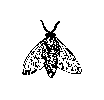
\epsfig{file=fly.eps}
%%\caption{A sample black and white graphic (.eps format).}
%%\end{figure}
%%
%%\begin{figure}
%%\centering
%%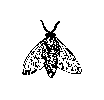
\epsfig{file=fly.eps, height=1in, width=1in}
%%\caption{A sample black and white graphic (.eps format)
%%that has been resized with the \texttt{epsfig} command.}
%%\end{figure}
%%
%%
%%As was the case with tables, you may want a figure
%%that spans two columns.  To do this, and still to
%%ensure proper ``floating'' placement of tables, use the environment
%%\textbf{figure*} to enclose the figure and its caption.
%%\begin{figure*}
%%\centering
%%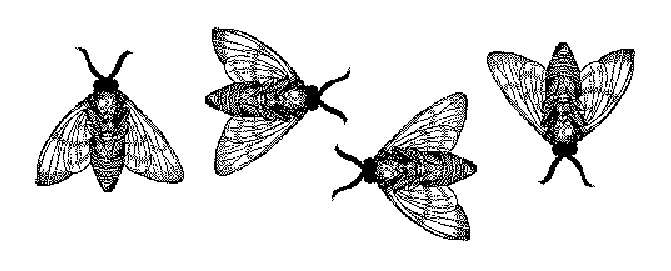
\epsfig{file=flies.eps}
%%\caption{A sample black and white graphic (.eps format)
%%that needs to span two columns of text.}
%%\end{figure*}
%%and don't forget to end the environment with
%%{figure*}, not {figure}!
%%
%%Note that, in this example file, {\textbf{.ps}} or {\textbf{.eps}} formats are
%%used; use
%%the \texttt{{\char'134}epsfig} or \texttt{{\char'134}psfig}
%%commands as appropriate for the different file types. We have also found that
%%PDF files (as `includable artwork') also works well.
%%
%%\begin{figure}
%%\centering
%%\psfig{file=rosette.ps, height=1in, width=1in,}
%%\caption{A sample black and white graphic (.ps format) that has
%%been resized with the \texttt{psfig} command.}
%%\vskip -6pt
%%\end{figure}
%
%\subsection{Theorem-like Constructs}
%Other common constructs that may occur in your article are
%the forms for logical constructs like theorems, axioms,
%corollaries and proofs.  There are
%two forms, one produced by the
%command \texttt{{\char'134}newtheorem} and the
%other by the command \texttt{{\char'134}newdef}; perhaps
%the clearest and easiest way to distinguish them is
%to compare the two in the output of this sample document:
%
%This uses the \textbf{theorem} environment, created by
%the\linebreak\texttt{{\char'134}newtheorem} command:
%\newtheorem{theorem}{Theorem}
%\begin{theorem}
%Let $f$ be continuous on $[a,b]$.  If $G$ is
%an antiderivative for $f$ on $[a,b]$, then
%\begin{displaymath}\int^b_af(t)dt = G(b) - G(a).\end{displaymath}
%\end{theorem}
%
%The other uses the \textbf{definition} environment, created
%by the \texttt{{\char'134}newdef} command:
%\newdef{definition}{Definition}
%\begin{definition}
%If $z$ is irrational, then by $e^z$ we mean the
%unique number which has
%logarithm $z$: \begin{displaymath}{\log e^z = z}\end{displaymath}
%\end{definition}
%
%Two lists of constructs that use one of these
%forms is given in the
%\textit{Author's  Guidelines}.
% 
%There is one other similar construct environment, which is
%already set up
%for you; i.e. you must \textit{not} use
%a \texttt{{\char'134}newdef} command to
%create it: the \textbf{proof} environment.  Here
%is a example of its use:
%\begin{proof}
%Suppose on the contrary there exists a real number $L$ such that
%\begin{displaymath}
%\lim_{x\rightarrow\infty} \frac{f(x)}{g(x)} = L.
%\end{displaymath}
%Then
%\begin{align*}
%l=\lim_{x\rightarrow c} f(x) &= \lim_{x\rightarrow c}{\left[ g{x} \cdot {\frac{f(x)}{g(x)}} \right]}\\
%&= \lim_{x\rightarrow c} g(x) \cdot \lim_{x\rightarrow c}{\frac{f(x)}{g(x)}} = 0\cdot L = 0, \\
%\end{align*}
%which contradicts our assumption that $l\neq 0$.
%\end{proof}
%
%Complete rules about using these environments and using the
%two different creation commands are in the
%\textit{Author's Guide}; please consult it for more
%detailed instructions.  If you need to use another construct,
%not listed therein, which you want to have the same
%formatting as the Theorem
%or the Definition\cite{salas:calculus} shown above,
%use the \texttt{{\char'134}newtheorem} or the
%\texttt{{\char'134}newdef} command,
%respectively, to create it.
%
%\subsection*{A {\secit Caveat} for the \TeX\ Expert}
%Because you have just been given permission to
%use the \texttt{{\char'134}newdef} command to create a
%new form, you might think you can
%use \TeX's \texttt{{\char'134}def} to create a
%new command: \textit{Please refrain from doing this!}
%The \textit{research4cacm} class file is quite complex and there is the
%risk that you may re\texttt{def}ine something. So, please remember, if you choose
%to use \texttt{{\char'134}def}, please be careful as recompilation will
%be, to say the least, problematic.
%
%% Additional text inserted here to expand the sample to 8 pages
%% ------------------------------------------------------------
%\section{More text}\label{sec:more-text}
%
%We also illustrate the effect of Laplacian smoothing on our medial
%axis approximation. For Laplacian smoothing we assume that we know the
%connectivity ordering of the sample points along the boundary curve
%$\partial O$. Every sample point has a predecessor and successor in
%this ordering. In Laplacian smoothing every sample point is displaced
%halfway toward the average of its predecessor and successor. This
%process is repeated iteratively.
%
%Typically, the input points sample a curve bounding a shape. In
%sample-based geometry processing, properties of shapes can be
%discovered by processing this point set, i.e., computing the
%Voronoi diagram, the Delaunay triangulation, or more complicated
%geometric structures. In Mesecina, such structures are offered for
%visualization as \emph{layers}. Currently, there are a total of 41
%layers available. Layers can be activated and deactivated, and
%properties like color, opacity, point size and line width are easily
%modifiable through the user interface.
%
%Unfortunately, the balls in $B_I$ are in general highly degenerate,
%i.e., many circles bounding such balls can pass through a single
%point. This makes the computation of the restricted power diagram of $B_I$,
%and thus the computation of the medial axis prone to
%numerical errors.
%
%This gives us an alternative, and numerically more stable way to
%compute the medial axis of the union of balls in $B_I$ under the
%condition that the smooth boundary $\partial O$ of $O$ is sampled
%sufficiently densely.
%
%The goal is to construct energy-efficient schedules, using lower processing speeds, while still
%guaranteeing a determined service. (2)~{\em Sleep states\/}: When a system is
%idle, it can be put into a low-power sleep state. One has to find out when to
%shut down a system, taking into account that a transition back to the active
%mode requires extra energy.
%
%{\bf Our contribution:} We present the first algorithm-based study of
%multi-processor speed scaling where jobs may have individual release dates and
%deadlines. Most of our paper concentrates on the offline scenario. In the first
%part of the paper we settle the complexity of the problem with unit size jobs.
%We may assume w.l.o.g.\ that $p(i)=1$, for all $i$.  We prove that if job
%deadlines are {\em agreeable\/}, an optimal multi-processor schedule can be
%computed in polynomial time. In practice, instances with agreeable deadlines
%form a natural input class where, intuitively, jobs arriving at later times may
%be finished later. Formally, deadlines are agreeable if, for any two jobs $i$
%and $i'$, relation $r(i)<r(i')$ implies $d(i)\leq d(i')$. We then show that if
%the jobs' release dates and deadlines may take arbitrary values, the energy
%minimization problem is NP-hard, even on two processors. For a variable number
%of processors, energy minimization is strongly NP-hard. Furthermore, for
%arbitrary release dates and deadlines we develop a polynomial time algorithm
%that achieves a constant factor approximation guarantee of
%$\alpha^\alpha2^{4\alpha}$.
%
%\begin{table*}[t]
%\caption{Inventory System Information}
%\centering
%\begin{tabular}{|r|c|c|c|c|c|c|c|c|c|}  \hline
% & No of & Lines & Mean & Dev Unit & PUT & Total & Fault & Files With & Pct With \\
% Rel & Files & of Code & LOC & Faults & Faults & Faults & Density & Any Faults & Any Faults \\ \hline
% 1  &  584 & 145,967 & 250 & 768 & 220 & 988 & 6.78 & 233 & 39.9 \\ \hline
% 2  &  567 & 154,381 & 272 & 172 & 28 & 200 & 1.30 & 88 & 15.5 \\ \hline
% 3  &  706 & 190,596 & 270 & 400 & 85 & 485 & 2.56 & 140 & 19.8 \\ \hline
% 4  &  743 & 203,233 & 274 & 292 & 35 & 327 & 1.61 & 114 & 15.3   \\ \hline
% 5  &  804 & 231,968 & 289 & 281 & 56 & 337 & 1.47 & 131 & 16.3  \\ \hline
% 6  &  867 & 253,870 & 293 & 288 & 51 & 339 & 1.34 & 115 & 13.3  \\ \hline
% 7  &  993 & 291,719 & 294 & 170 & 37 & 207 & 0.71 & 106 & 10.7  \\ \hline
% 8  & 1197 & 338,774 & 283 & 375 & 113 & 488 & 1.45 & 148 & 12.4 \\ \hline
% 9  & 1321 & 377,198 & 286 & 346 & 88 & 434 & 1.16 & 151 & 11.4  \\ \hline
% 10 & 1372 & 396,209 & 289 & 202 & 43 & 245 & 0.62 & 112 & 8.2  \\ \hline
% 11 & 1607 & 426,878 & 266 & 174 & 106 & 280 & 0.66 & 114 & 7.1  \\ \hline
% 12 & 1740 & 476,215 & 274 & 192 & 81 & 273 & 0.57 & 120 & 6.9  \\ \hline
% 13 & 1772 & 460,437 & 260 & 88 & 39 & 127 & 0.28 & 71 & 4.0 \\ \hline
% 14 & 1877 & 482,435 & 257 & 164 & 71 & 235 & 0.49 & 95 & 5.1  \\ \hline
% 15 & 1728 & 479,818 & 278 & 251 & 54 & 305 & 0.64 & 120 & 6.9  \\ \hline
% 16 & 1847 & 510,561 & 276 & 181 & 93 & 274 & 0.54 & 116 & 6.3  \\ \hline
% 17 & 1950 & 538,487 & 276 & 188 & 65 & 253 & 0.47 & 122 & 6.3  \\ \hline
%\end{tabular}
%\label{rel-dens}
%\end{table*}
%
%Denote the bidding function as $b(v)$. We conjecture that the bidding
%function is monotonically increasing (we can verify that this is true), so
%that the reverse bidding function exists and is increasing, denoted as $%
%\eta \left( b\right) $. If one's rivals bid according to such a bidding
%function, we can write out its probability of winning $j$th share as%
%\[
%P_{j}\left( b\right) =\left( _{n-j}^{n-1}\right) F\left( \eta \left(
%b\right) \right) ^{n-j}\left[ 1-F\left( \eta \left( b\right) \right) \right]
%^{j-1}
%\]%
%In equilibrium, the winning probability for a bidder with valuation $v$ is%
%\[
%P_{j}\left( v\right) =\left( _{n-j}^{n-1}\right) F\left( v\right) ^{n-j}
%\left[ 1-F\left( v\right) \right] ^{j-1}
%\]
%
%Denote $v_{0}\in \left[ \underline{v},\bar{v}\right] $ as a reserve price
%(minimal bid) set by the auctioneer. Clearly, an advertiser
%with $v<v_{0}$ will not bid.
%
%Denote
%\[
%\int_{v_{0}}^{\overline{v}}P_{j}\left( v\right) \left[ v-\frac{1-F(v)}{f(v)}%
%\right] f(v)dv\equiv \alpha _{j}
%\]%
%and let $\alpha _{m+1}=0$ for notation convenience. $\alpha _{j}$\ can be
%interpreted as the marginal return of $j$th share. The coefficients ($\alpha
%_{j} $) are generally determined by the distribution function, the
%reservation price, and the number of bidders.
%
%From the above Proposition 1, we can see that the expected profit of the
%auctioneer is a linear function of share sizes. Intuitively, one would want
%to allocate as much resource as possible to the share with the highest
%marginal return. Thus the optimal share structure is ultimately determined by
%the rank order of these marginal returns. In below, we show the conditions under
%which the marginal return of the largest share is the highest such that
%providing just one grand share is optimal.
%
%\section{Some Additional Text}
%
%Table~\ref{rel-dens} provides information on the inventory system.
%We observed that, after the first release, less than 20\% of the files contained any faults
%at all, discovered at any stage of development.
%Therefore, we reasoned, if we could identify these files, substantial
%effort could be saved if testers could target these files for particular scrutiny.
%
%All three systems used an integrated version control/change management
%system that required a {\em modification request} or MR to be written
%any time a change was to be made to the system.
%An MR, which is most commonly written by a developer or tester, may
%identify either (1) a problem or issue found during internal project testing or
%reported by a customer or (2) a required or requested change, such
%as a system enhancement or maintenance update.
%
%MRs contain a great deal of information, including a written description
%of the reason for the proposed change and a severity rating of 1 through
%4 characterizing the importance of the proposed change.
%If the request results in an actual change, the MR records the file(s)
%that are changed or added to the system and the specific lines of code
%that are added, deleted, or modified.
%It also includes such information as the date of the change and the
%development stage at which the change was made.
%
%Most projects begin MR data collection at the time that the system test phase begins for the
%first release, and this was the case for the provisioning system used in our case studies.
%The inventory system began data collection far earlier, at the requirements stage, and almost
%three quarters of the reported faults were identified during unit testing.
%Unlike system testing, which is typically done by professional testers whose sole job function
%is to develop and run test cases once the system has been fully integrated, unit testing
%is generally performed by developers while they are creating individual files.
%In addition, the system test process tends to be far more carefully controlled than the unit
%testing phase.
%
%One of the reasons why the testing process has gained such a
%denotative importance is the fact that it consumes even
%50\% of the expended effort on software development
%\cite{Pressman2002}. Thus, the software testing activity is
%a critical element on the search of quality assurance of a
%software product, aiming to make it more reliable.
%
%\textbf{Learning.} Between periods 0 and 1 seller $M$ receives information
%form his buyers. We aggregate the information as follows: Let $\mu _{i}$
%denote the measure of buyers who buy product $i\in \left\{ l,h\right\} $
%from seller $M$ in period 0. Seller $M$ receives a random signal $%
%y_{i}\left( x_{i}\right) \in \left\{ -1,0,1\right\} $ on the type of each
%product $i\in \left\{ l,h\right\} $ between periods 0 and 1, where
%\begin{eqnarray*}
%\Pr \left( y_{i}\left( x_{i}\right) =0\mid x_{i}\right) &=&1-\mu _{i}, \\
%\Pr \left( y_{i}\left( x_{i}\right) \in \left\{ -1,1\right\} \mid
%x_{i}\right) &=&\mu _{i}.
%\end{eqnarray*}%
%We can interpret a signal of $0$ as containing no information, or simply the
%failure to receive an informative signal. Given that the seller receives a
%relevant signal, the probability of the signal being correct is:
%\[
%\Pr \left( y_{i}\left( x_{i}\right) =x_{i}\mid y_{i}\left( x_{i}\right) \in
%\left\{ -1,1\right\} ,x_{i}\right) =\frac{1}{2}+\gamma ,
%\]%
%where $\gamma \in \left[ 0,\frac{1}{2}\right] $. We can interpret $\gamma $\
%as the informativeness of the signal. The event tree in Figure 2 summarizes
%the signal structure where $x_{i}^{\prime }\neq x_{i}$.
%
%Given the probabilistic structure, we view this type of system as a
%mechanism that computes the posterior beliefs for each product $i$ based on
%the signal $y_{i}$ and reports them only to the buyers who have bought from
%him in period 0. The posterior for product $i$ given signal $y_{i}$ will be
%denoted by
%\[
%\alpha _{i}\left( y_{i}\right) \equiv \Pr \left( x_{i}=1\mid y_{i}\right) .
%\]
%
%A performance analysis of distributing QoS parameters over multiple
%entities able to communicate together has been performed in this paper.
%In this study, we compared the amount of data exchanged in two scenarios
%differentiated on the basis of the negotiation approach in use. Our
%analysis points out that the HD architecture seems to be an alternative
%operator-centric solution to improve QoS management on network side. In
%fact, data exchanged on network side in HD architecture scenario is less
%than in UMTS scenario. However, this solution increases the amount of
%data exchanged on end terminal side. This amount can be reduced by
%adopting network assisted or controlled QoS management approaches.
%Noticed that this optimization can also be applied during handover
%management. We are currently assessing the performance of our
%optimization in such a case.
%
%\begin{eqnarray}
%    &&B_{UMTS\_R5}^{Terminal} = 4*S_{QoSd} + 184 \\
%    &&B_{UMTS\_R5}^{GGSN} = 12*S_{QoSd} + 552\\
%    &&B_{UMTS\_R5}^{SGSN} = 2*(l + 2)*(S_{QoSd} + 46)\\
%    &&B_{UMTS\_R5}^{RNC} = 2*S_{QoSd} + 92 \\
%    &&B_{UMTS\_R5}^{Network} = (11 + 2*l)*S_{QoSd} + 874 \\ \nonumber
%    %\end{eqnarray}
%    %\begin{eqnarray}
%    %&&B_{DAIDALOS}^{Terminal} = 3*S_{QoSd} + 138 \\
%    %&&B_{ DAIDALOS }^{ANQoSB} = 2*(l + 3)*(S_{QoSd} + 46\\
%    %&&B_{ DAIDALOS }^{MMSP} =12*S_{QoSd} +552\\
%    %&&B_{ DAIDALOS }^{AR} = 2*l*(S_{QoSd} + 46) \\
%    %&&B_{ DAIDALOS }^{Network} = 2*(l + 6)*(S_{QoSd} + 46) \\ \nonumber\\
%    &&B_{HD}^{Terminal} = 3*S_{QoSd} + l*S_{RM} + (l + 3)*46\\
%    &&B_{HD}^{OM} = 3*S_{QoSd} + S_{OM} + 184\\
%    &&B_{HD}^{IPAM} = 3*S_{QoSd} + S_{OM} + l*(S_{RM}{} \nonumber \\
%    & & {} + S_{IPAM}) + (l + 4)*46  \\
%    &&B_{HD}^{RM} = 4*S_{QoSd} + 2*S_{RM} + S_{IPAM} + 276\\
%    &&B_{HD}^{Network} = 8*S_{QoSd} + S_{OM} + l*S_{IPAM} {} \nonumber \\
%    & & {}+ 2*S_{RM} + (2*l + 9)*46
%\end{eqnarray}%}
%
%We begin by describing the notation used
%in this paper.
%The network is represented as the AS graph
%$G = (V, E)$, where each node $v \in V$
%corresponds to one AS, and each edge $\{u,v\} \in E$
%corresponds to a \emph{BGP session} between ASes
%$u$ and $v$, meaning that these ASes are physically connected
%and share route advertisements.
%We assume that links between ASes are reliable FIFO message queues with
%arbitrary delays; this accounts for network asynchrony. At most one link
%is assumed to exist between ASes, and all the internal and border
%routers of an AS are condensed into one node (or one point of
%routing-policy control). A path $P$ is a sequence of nodes $v_1 v_2
%\cdots v_k$ such that $\{v_i, v_{i+1}\} \in E$; we write $v \in P$ if
%path $P$ traverses node $v$. Paths can be concatenated with other nodes
%or paths; \emph{e.g.}, if $P = u \cdots v$, $Q = v \cdots w$, and
%$\{w,d\} \in E$, we may write $PQd$ to represent the path starting at
%node $u$, following $P$ to node $v$, then following $Q$ to node $w$, and
%finally traversing the edge $(w, d)$. We assume that paths are directed
%from source to destination.
%BGP, at a schematic level, computes routes using the following iterative
%process: (1) Nodes receive \emph{route advertisements} from their
%neighbors, indicating which destinations are reachable and by what
%routes; (2) for each destination, a node chooses the best route from
%those available, based on local policy; (3) if the current route to a
%given destination has changed, an advertisement is sent to neighboring
%nodes.
%
%We say the network has converged when each AS $v \in V$ is assigned a
%path $\pi(v)$ to the destination, such that the assignment is
%\emph{stable}, \emph{consistent} and {\em safe}. By consistent, we mean
%that the paths form a forwarding tree to the destination; if $\pi(v) =
%vuP$, then $\pi(u) = uP$. By stable, we mean that $\pi(v)$ is the
%``best'' available route for each node $v$, given the other nodes' path
%assignments, where ``best'' is determined by node $v$'s routing policy;
%that is, if $\pi(v)=v\pi(u)$, there is no other node $w$ such that the
%path $v\pi(w)$ is more preferred at $v$ than $\pi(v)$.
%
%In this simple example, we note that the router counter does not get propagated beyond the
%immediate neighboring pivot. In the detection phase, node {\em B} advertises ({\em BD}:1),
%which does not need to be readvertised in the next iteration since {\em B}  receives ({\em CD}:1) thereafter.
%As the counter is propagated together with route advertisements, this implies that no
%further updates to it will take place in the stable phase.
%
%Considering differences and similarities between both of them,
%many open questions are discussed about AO testing, the importance
%of the development of a testing model for Aspect--Oriented Programs
%(AOPs), and also the inclusion of a potential fault on the model
%proposed by Alexander \cite{Alexander2004}.
%
%On an algorithmic level there are two mechanisms to save energy.  (1)~{\em Speed
%scaling\/}: Microprocessors currently sold by chip makers such as AMD and Intel
%are able to operate at variable speed. The higher the speed, the higher the
%power consumption is. Speed scaling techniques dynamically adjust the speed of a
%processor executing a set of computing tasks. The goal is to construct
%energy-efficient schedules, using lower processing speeds, while still
%guaranteeing a determined service. (2)~{\em Sleep states\/}: When a system is
%idle, it can be put into a low-power sleep state. One has to find out when to
%shut down a system, taking into account that a transition back to the active
%mode requires extra energy.
%
%\subsection{A subsection with more text}
%
%Some OO software testing facilities regarding procedural are
%presented by McGregor \cite{McGregor1996}: i) methods and classes
%interfaces are explicitly defined; ii) lesser number of testing
%cases to coverage are resultant, due to the reduced number of
%parameters; and iii) reuse of testing cases due to the presence of
%the inheritance characteristic. Alexander \cite{Alexander2004} presents specific issues to testing
%process over AO paradigm: How to adequately test aspect-oriented
%process?
%
%McGregor \cite{McGregor1996} also points out some disadvantages
%which must be considered, like: i) the class correctness
%evaluation, complicated by the presence of information
%encapsulation; ii) the testing management, obstructed by the
%multiple entry points (methods) in one class; and iii) object
%iterations, expanded by polymorphism and dynamic binding.
%
%Zhao \cite{Zhao2003} proposes a unit testing approach based on
%data flow to test AO programs. This approach tests two kinds of
%units for AO programs: aspects as modular units that implement
%crosscutting concerns, and classes whose behavior could be
%affected by one or more aspects. To every unit, three levels of
%distinct tests are applied: intra-module, inter-module, and
%intra-aspects or intra-classes. Def-use pairs are computed using
%Control Flow Graphs (CFG) to define what interactions between
%aspects and classes must be tested.
%
%\textit{Case 2:} In this case we assume $a(i+k) < a(i+1)$ and $b(i+k)\leq
%b(i+1)$. Our goal is to swap jobs $i+1$ and $i+k$.
%To this end we exchange start and finishing times of jobs $i+1$ and $i+k$ as
%follows. Let $a'(i+k) := a(i+1)$, $b'(i+k) := b(i+1)$ and $a'(i+1):=a(i+k)$,
%$b'(i+1):=b(i+k)$. We can now execute job $i+1$ on processor $(i+1) \bmod m$
%(where $i+k$ was scheduled earlier) and job $i+k$ on processor $j$. The new
%schedule is feasible since $r(i+1)\leq r(i+k)$ and $d(i+1) \leq d(i+k)$ by the
%agreeable deadline property. The energy consumption did not change because the
%total energy consumed by $i+1$ and $i+k$ remains unchanged for they have unit
%size.
%
%Like some of the characteristics found
%on object oriented languages reduce the probability of some
%errors, others favor the appearance of new categories of
%the same \cite{Binder1999}. Among the favoring characteristics, it
%can be cited the encapsulation, polymorphism and dynamic binding.
%
%\textit{Case 3:} For the last case we assume \hbox{$a(i+k) < a(i+1)$} but
%$b(i+k)>b(i+1)$. We can now exchange the start times
%of jobs $i+1$ and $i+k$ by setting $a'(i+1):= a(i+k)$ and $a'(i+k):= a(i+1)$.
%Since start times are exchanged, we can now swap the complete work assignment on
%processor $(i+1) \bmod m$ after (and including) job $i+k$ with the work
%assignment on processor $j$ after (and including) job $i+1$. The schedule is
%feasible since (by agreeable deadlines) $r(i+1) \leq r(i+k)$. The power
%consumption of jobs $i+1$ and $i+k$ in the original schedule is
%$(b(i+1)-a(i+1))^{1-\alpha}+(b(i+k)-a(i+k))^{1-\alpha}$ while we have
%$(b(i+1)-a(i+k))^{1-\alpha}+(b(i+k)-a(i+1))^{1-\alpha}$ in the modified
%schedule. By the convexity of the power function the latter expression is
%smaller because $a(i+k) < a(i+1)$.
%
%When analyzing {\em CRR\/} on ${\cal J'}$, rather than the optimal schedules
%constructed in step~2 of the algorithm, we will consider schedules generated
%according to the {\em Average Rate (AVR)} algorithm by Yao.
%This algorithm sets processor speeds according to job densities. For any
%processor $j$ and time $t$, where $1\leq j \leq m$ and $t\in [0,T)$, let
%$c_{kj}(t)$ be the number of jobs from class $C_k$ active at time $t$ that have
%been assigned by {\em CRR\/} to processor $j$. Set the speed of processor $j$ at
%time $t$ to
%
%\begin{equation}\label{eq:sk}
%    s_j(t) = \sum_{k\geq 0} c_{kj}(t)\Delta/2^k.
%\end{equation}
%
%Sequencing available jobs on processor $j$ according to the {\em Earliest
%Deadline\/} policy yields, not surprisingly, an extremly feasible schedule. Let $S'_{{\mathit AVR},j}$ be the
%resulting schedule on processor $j$ and $E'_{AVR,j}$ the energy consumption of
%$S'_{\mathit AVR,j}$. As {\em CRR\/} computes an optimal schedule for each
%processor, its total energy $E'_{CRR}$ is bounded by
%$$
%    E'_{CRR} \leq \sum_{j=1}^m E'_{AVR,j}.
%$$
%We next estimate the energy volumes $E'_{AVR,j}$,
%$1\leq j \leq m$. To this end we consider two energy bounds. Firstly, suppose
%that job $i'\in {\cal J'}$ is processed at speed $1/(d(i')-r(i'))$ throughout
%its active interval. The minimum energy necessary to complete the job is
%$(d(i')-r(i'))^{1-\alpha}$ and hence the minimum energy necessary to complete
%all jobs $i'\in {\cal J'}$ is at least
%\begin{equation}\label{eq:emin}
%    E'_{\min}
%    = \sum_{i'\in {\cal J'}} (d(i')-r(i'))^{1-\alpha}
%    = \sum_{k\geq 0}\sum_{i'\in C_k} (2^k/\Delta)^{1-\alpha}.
%\end{equation}
%
%Secondly, we consider the single processor schedule $S'_{\mathit AVR}$
%constructed by {\em AVR\/} for ${\cal J'}$.  More specifically, at time $t$ the
%speed is set to
%
%\begin{equation}\label{eq:st}
%    s(t) = \sum_{k\geq 0} c_k(t)\Delta/2^k.
%\end{equation}
%
%%
%\begin{proof}
%On processor $j$ we schedule the jobs in $S_j$ in increasing order of job
%number. Thus the jobs are scheduled in non-decreasing order of deadlines.  We
%first consider any job $i\in S_j$ with $p(i) \leq L(i)/m$ and then any $i\in
%S_j$ with $p(i) > L(i)/m$. In both cases we will prove that the job is finished
%by its deadline.
%
%Fix any $i\in S_j$ with $p(i) \leq L(i)/m$. We will show that after the initial
%speed setting in step~1 of the speed function definition, the job is finished by
%$d(i)$. As the speed can only increase in the adjustment step~2, the lemma then
%holds for this job $i$. Let $k$ be the largest integer such that
%$\lambda_k^j\leq i$. By time $d(\lambda^j_k)$ a total load of
%
%\begin{align}
%    \sum_{l=1}^{k}&\left(2-{1\over m}\right) s^j_l (d(\lambda^j_l) -
%    d(\lambda^j_{l-1}))\nonumber\\
%    &=  \left(2-{1\over m}\right)\sum_{l=1}^{k} {1\over m}
%        {L(\lambda_l^j)-L(\lambda_{l-1}^j)\over d(\lambda_l^j)-d(\lambda_{l-1}^j)}
%        (d(\lambda^j_l) - d(\lambda^j_{l-1}))\nonumber\\
%    &= \left(2-{1\over m}\right) L(\lambda_k^j)/m\label{eq:L1}
%\end{align}
%is completed on processor $j$. If $i>\lambda_k^j$, then between time
%$d(\lambda^j_k)$ and $d(i)$ a load of
%
%\begin{multline}    \label{eq:L2}
%    \left(2-{1\over m}\right) s^j_{k+1} (d(\lambda^j_{k+1}) -
%    d(\lambda^j_k))\\
%    = \left(2-{1\over m}\right){1\over m} {L(\lambda_{k+1}^j)-L(\lambda_k^j)\over
%        d(\lambda_{k+1}^j)-d(\lambda_k^j)} (d(i) - d(\lambda^j_k))\\
%    \geq \left(2-{1\over m}\right){1\over m} {L(i)-L(\lambda_k^j)\over d(i)-d(\lambda_k^j)}
%        (d(i) - d(\lambda^j_k))\\
%    = \left(2-{1\over m}\right) (L(i)-L(\lambda_k^j))/m
%\end{multline}
%is completed. The inequality follows from the definition of $\lambda^j_{k+1}$.
%Combining (\ref{eq:L1}) and (\ref{eq:L2}) we find that a total load of at least
%$(2-{1\over m})L(i)/m$ is finished on processor $j$ by time $d(i)$. It remains
%to argue that the total processing requirement of jobs scheduled on processor
%$j$ before job $i$ and including $p(i)$ is at most $(2-{1\over m})L(i)/m$.  To
%this end consider the event when {\em EDL\/} assigns job $i$ to processor $j$.
%As the job is placed on the least loaded processor, just after the assignment
%processor $j$ has a load of at most ${1\over m} \sum_{i'<i}p(i') + p(i) \leq
%(2-{1\over m})L(i)/m$, and we are done because jobs assigned to processor $j$ at
%a later stage are scheduled after job $i$.
%
%Next we examine a job $i$ with $p(i) > L(i)/m$. After the speed adjustment in
%step~2 of the speed function definition, processor $j$ runs at a speed of at
%least $(2-{1\over m}) p(i)/d(i)$ throughout $[0,d(i))$. Thus a total work of at
%least $(2-{1\over m})p(i)$ gets finished by $d(i)$. Again, when {\em EDL\/}
%assigns job $i$ to processor $j$, the total load on the processor is upper
%bounded by ${1\over m} \sum_{i'<i}p(i') + p(i) \leq (2-{1\over m})p(i)$ and this
%is indeed the total work of jobs scheduled on processor $j$ up to (and
%including) job $i$.
%\end{proof}
%
%We compare the energy incurred by the speed function to the energy of an optimal
%solution.  Let
%
%$$
%    E_j^1 = \sum_{l=1}^{l_j} (s^j_l)^{\alpha} (d(\lambda^j_l) - d(\lambda^j_{l-1})).
%$$
%
%This expression represents the energy used by our speed function on processor
%$j$ after the initial setting when speeds are reduced by a factor of $2-{1\over
%m}$.
%
%Given an optimal schedule, let $s_{l,{\rm opt}}$ be the average speed of the $m$
%processors during the time interval $[d(\lambda^j_{l-1}), d(\lambda^j_l))$, for
%$l=1, \ldots, l_j$. By the convexity of the power function, the total energy
%used by the optimal solution is
%
%$$
%    E_{{\rm OPT}}
%    \geq m \sum_{l=1}^{l_j} (s_{l,{\rm opt}})^{\alpha} (d(\lambda^j_l)- d(\lambda^j_{l-1})).
%$$
%
%The speeds $s_{l,{\rm opt}}$ must satisfy the constraint that at time
%$d(\lambda^j_k)$ a load of at least $L(\lambda^j_k)$ is completed, for $k=1,
%\ldots, l_j$. In the following let $\delta^j_l= d(\lambda^j_l)-
%d(\lambda^j_{l-1})$.
%%We next show that the speeds $s^j_l$, with $1\leq l \leq
%%l_j$, defined in (\ref{eq:speed}) minimize the function $f(x_1,\ldots,x_{l_j}) =
%%m \sum_{l=1}^{l_j} x_l^{\alpha} \delta^j_l$ subject to the constraint
%
%\begin{equation}\label{eq:const}
%    m \sum_{l=1}^k x_l \delta^j_l \geq L(\lambda^j_k),
%\end{equation}
%for $k=1, \ldots, l_j$.  Suppose $(y_1, \ldots, y_{l_j})$ with  $(y_1, \ldots,
%y_{l_j}) \neq (s^j_1, \ldots, s^j_{l_j})$ is an optimal solution. Note that
%
%\begin{equation}\label{eq:load}
%    m \sum_{l=1}^k s^j_l \delta^j_l = L(\lambda^j_k),
%\end{equation}
%for $k=1, \ldots, l_j$. Thus there must exist a $k$ with $y_k > s_k^j$: If $y_l
%\leq s_l^j$ held for $l=1, \ldots, l_j$, then there would be a $k'$ with $y_{k'}
%< s_{k'}^j$ and hence $m \sum_{l=1}^{k'} y_l^{\alpha} \delta^j_l <
%L(\lambda^j_{k'})$, resulting in a violation of constraint (\ref{eq:const}) for
%$k=k'$.  Let $k_1$ be the smallest index such that $y_{k_1} > s_{k_1}^j$. We
%have $y_l = s^j_l$, for $l=1, \ldots, k_1-1$ since otherwise, using the same
%argument as before, constraint (\ref{eq:const}) would be violated for $k=k_1-1$.
%Let $k_2$ with $k_2 > k_1$ be the smallest index such that $y_{k_1}> y_{k_2}$.
%Such an index exists because otherwise the invariant implies $y_l
%> s^j_l$, for $l=k_1, \ldots, l_j$, and we find $m \sum_{l=1}^{l_j} y_l
%\delta^j_l > L(\lambda^j_{l_j})$. In this case we could reduce $y_{l_j}$,
%achieving a smaller objective function value $f$ and hence a contradiction to
%the optimality of the $y_l$, $1\leq l \leq l_j$.
%% ------------------------------------------------------------

%\section{Conclusions}
%This paragraph will, effectively, end the body of this sample document.
%You might still have Acknowledgments or an Appendix in your \textit{original}
%conference article, however, do remember
%(as stated in the Introduction) \textit{Research Highlights}
%are purposefully edited so that they appeal to a broader community.
%Whilst, for example, explicit proofs of theorems are appropriate, and welcomed, in an
%Appendix section for a \textit{Proceedings}, they are inappropriate in the context
%of a \textit{magazine}.
%
%There is still the Bibliography to deal with; and
%we will make a disclaimer about that here: with the exception
%of the reference to the \LaTeX\ book, the citations in
%this paper are to articles which have nothing to
%do with the present subject and are used as
%examples only.
%
%Most authors will avail of a \textit{bibliography database} (\texttt{.bib})
%and \texttt{{\char'134}cite} the key values therein. The most appropriate
%\textit{bibliography style file} (\texttt{.bst}) to use is the \texttt{abbrv} style.
%ACM endorses the use of a \texttt{.bib} and the \texttt{abbrv} style in order
%to produce the references. However, because the number of references for a
%\textit{Researchh Highlights} article is reduced, we have no
%problem with authors choosing, instead, to enter their references \textit{directly} using
%a \texttt{{\char'134}bbl}.

%ACKNOWLEDGMENTS are optional
\section{Acknowledgments}
Special thanks to Martijn Donders and Rob Bloemer for their cryptographic support.


% The following two commands are all you need in the
% initial runs of your .tex file to
% produce the bibliography for the citations in your paper.
\bibliographystyle{abbrv} % standard abbrv style
\bibliography{bibs4cacm,article,misc}  % substitute the name of 'your' Bibliography here
% You must have a proper ".bib" file
% and remember to run:
% latex bibtex latex latex (in that particular order) in order to resolve all the 'numerical values'
% be they for figures, equation numbers, references, footnotes, etc. etc.
%
\balancecolumns
% That's all folks! % GM Sept. 2008
\end{document}
